\documentclass[tikz]{standalone}

\usepackage{tikz}
\usepackage{ifthen}
\pgfdeclarelayer{back}
\pgfsetlayers{back,main}

%
% Customize colors
%
\definecolor{chapter-color}{cmyk}{1, 0.50, 0, 0.25}
\definecolor{link-color}{cmyk}{1, 0.50, 0, 0.25}
\definecolor{cite-color}{cmyk}{0, 0.7, 0.9, 0.2}
\definecolor{codegreen}{rgb}{0,0.6,0}
\definecolor{codegray}{rgb}{0.5,0.5,0.5}
\definecolor{codepurple}{rgb}{0.58,0,0.82}
\definecolor{backcolour}{rgb}{0.95,0.95,0.92}
\definecolor{codebgcolor}{RGB}{129, 139, 152}
\definecolor{codehighlightcolor}{RGB}{255, 230, 153}
%\definecolor{codegreen}{RGB}{0, 153, 0}
%\definecolor{codegray}{RGB}{127, 127, 127}
\definecolor{codeblue}{RGB}{102, 214, 237}
\definecolor{codekeyword}{RGB}{249, 36, 114}
\definecolor{codecomment}{RGB}{127, 127, 127}
\definecolor{backcolor}{RGB}{242, 242, 235}
\definecolor{linkcolor}{RGB}{102, 0, 0}
\definecolor{corange}{RGB}{255, 70, 0}
\definecolor{cyellow}{RGB}{209, 153, 0}
\definecolor{cblue}{RGB}{64, 128, 255}
\definecolor{cbrown}{RGB}{153, 102, 51}
\definecolor{cpink}{RGB}{255, 0, 255}
\definecolor{cred}{RGB}{255, 64, 0}
\definecolor{cgreen}{RGB}{0, 191, 0}
\definecolor{clightblue}{RGB}{191, 217, 255}
\definecolor{cturquois}{RGB}{0, 255, 255}
\definecolor{cpurple}{RGB}{128, 0, 255}
\definecolor{clightgreen}{RGB}{175, 255, 175}
\definecolor{clightgray}{RGB}{211, 211, 211}
\definecolor{clightpink}{RGB}{255, 175, 255}
\definecolor{cdarkblue}{RGB}{0, 0, 255}
\definecolor{cdarkred}{RGB}{255, 0, 0}
\definecolor{cdarkgreen}{RGB}{0, 255, 0}
\definecolor{cgray}{RGB}{153, 153, 153}

\definecolor{myblue}{RGB}{55, 126, 184}
\definecolor{myorange}{RGB}{255, 127, 0}
\definecolor{myred}{RGB}{228, 26, 28}
\definecolor{mypurple}{RGB}{152, 78, 163}
\definecolor{mygreen}{RGB}{77, 175, 74}
\definecolor{myyellow}{RGB}{255, 255, 51}
\definecolor{mybrown}{RGB}{166, 86, 40}
\definecolor{mypink}{RGB}{166, 86, 40}
\definecolor{mygray}{RGB}{153, 153, 153}


\colorlet{colorL0}{myorange}
\colorlet{colorL1}{mygreen}
\colorlet{colorL2}{myred}
\colorlet{colorL3}{mypurple}

\begin{document}

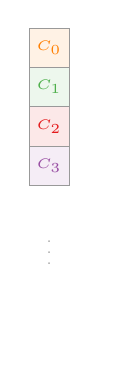
\begin{tikzpicture}

\tikzstyle{every node}=[font=\tiny, text=gray]

\def\x{1}%
\def\y{0}%
\coordinate (A1) at (\x*0.5+0.0,3.5-\y*0.5);
\coordinate (B1) at (\x*0.5+0.5,4.0-\y*0.5);
\draw[color=white, fill=white, very thin] (A1) rectangle (B1) node[midway, color=white]{};

\def\x{0}%
\foreach \y in {0,...,7} {
  \coordinate (A1) at (\x*0.5+0.0,3.5-\y*0.5);
  \coordinate (B1) at (\x*0.5+0.5,4.0-\y*0.5);

  \ifthenelse{\y=0}{
    \draw[color=mygray, fill=colorL0!10, very thin] (A1) rectangle (B1)
        node[midway, color=colorL0]{$C_{\y}$};
  }{
    \ifthenelse{\y=1}{
      \draw[color=mygray, fill=colorL1!10, very thin] (A1) rectangle (B1)
          node[midway, color=colorL1]{$C_{\y}$};
    }{
      \ifthenelse{\y=2}{
        \draw[color=mygray, fill=colorL2!10, very thin] (A1) rectangle (B1)
            node[midway, color=colorL2]{$C_{\y}$};
      }{
        \ifthenelse{\y=3}{
          \draw[color=mygray, fill=colorL3!10, very thin] (A1) rectangle (B1)
              node[midway, color=colorL3]{$C_{\y}$};
        }{
          \ifthenelse{\y=5}{
            \draw[color=white, very thin] (A1) rectangle (B1)
                node[midway, color=mygray]{$\vdots$};
          }{
            \draw[color=white, opacity=0.0, very thin] (A1) rectangle (B1)
                  node[midway, color=mygray]{};
          };
        };
      };
    };
  };
};

\end{tikzpicture}

\end{document}